\documentclass[DaoFP]{subfiles}
\begin{document}
\setcounter{chapter}{15}

\chapter{单子与伴随}

\section{弦图}

一条线将平面分割。我们可以将其视为将平面分割,或者将平面的两半连接起来。

一个点将一条线分割。我们可以将其视为将两条半线分开,或者将它们连接在一起。

这是一个图表,其中两个类别表示为点,两个函子表示为箭头,自然变换表示为双箭头。

\[
\begin{tikzpicture}[column sep=huge]
\def \xa{-1.2};
\def \xb{0};
\def \xc{1.2};
\def \ya{-1};
\def \yb{0};
\def \yc{1};

\node(c) at (\xa, \yb) {};
\node[left] at (c) {$\mathcal{C}$};
\filldraw[black] (c) circle (1 pt);
\node(d) at (\xc, \yb) {};
\node[right] at (d) {$\mathcal{D}$};
\filldraw[black] (d) circle (1 pt);

\draw [->] (c) to [out=60,in=120] node[midway, above]{$G$}(d);
\draw [->] (c) to [out=-60,in=-120] node[midway, below]{$F$}(d);

\node(mup) at (\xb, \yc -0.5) {};
\node(mdn) at (\xb, \ya + 0.5) {};
\draw[->, -{Implies}, double, double distance=2pt] (mdn) -- node[midway, left]{$\alpha$} (mup);
\end{tikzpicture}
\]

但同样的想法可以通过将类别表示为平面的区域,函子表示为区域之间的线,自然变换表示为连接线段的点来表示。

这个想法是,函子总是在一对类别之间进行,因此可以将其绘制为它们之间的边界。自然变换总是在一对函子之间进行,因此可以将其绘制为连接两条线段的点。

\[
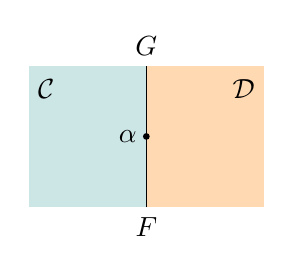
\begin{tikzpicture}
\def\x{0};
\def\xl{-1.5};
\def\xr{1.5};


\def \ya{0.8};
\def \yb{1.7};
\def \yc{2.6};
\def \yt {2.3};

\filldraw[fill=blue!50!green!20, draw=white] (\xl, \ya) rectangle (\x, \yc);
\filldraw[fill=orange!30, draw=white] (\x, \ya) rectangle (\xr, \yc);

\node[below] (a) at (\x, \ya) {$F$};
\node(b) at (\x, \yb) {};
\node [above] (c) at (\x, \yc) {$G$};

\node(l)[right] at (\xl, \yt) {$\mathcal{C}$};
\node(r)[left] at (\xr, \yt) {$\mathcal{D}$};


\filldraw[black] (b) circle (1 pt);
\node [left] at (b) {$\alpha$};

\draw (a)  -- (c);

\end{tikzpicture}
\]

这是一个\emph{弦图}的例子。你从下到上、从左到右阅读这样的图表(想象$(x, y)$坐标系)。

图表的底部显示了从$\mathcal{C}$到$\mathcal{D}$的函子$F$。图表的顶部显示了在同一对类别之间的函子$G$。转换发生在中间,自然变换$\alpha$将$F$映射到$G$。

在Haskell中,这个图表被解释为两个自函子之间的多态函数:
\begin{haskell}
alpha :: forall x. F x -> G x
\end{haskell}

到目前为止,使用这种新的视觉表示似乎并没有带来太多好处。但让我们将其应用到更有趣的东西上:自然变换的垂直组合:
\[
\begin{tikzcd}[column sep=huge]
\mathcal{C}
  \arrow[bend left=60]{rr}[name=U, label=above:$H$]{}
  \arrow[]{rr}[name=M, label={[xshift=15pt, yshift=-5pt]:$G$}]{} 
  \arrow[bend right=60]{rr}[name=D, label=below:$F$]{} 
 &&
\mathcal{D}
  \arrow[shorten <=8pt, shorten >=8pt,Leftarrow, to path={(U) -- node[label=left:$\beta$] {} (M)}]{}
  \arrow[shorten <=8pt, shorten >=8pt,Leftarrow, to path={(M) -- node[label=left:$\alpha$] {} (D)}]{}
\end{tikzcd}
\]

相应的弦图显示了两个类别和它们之间的三个函子,由两个自然变换连接。
\[
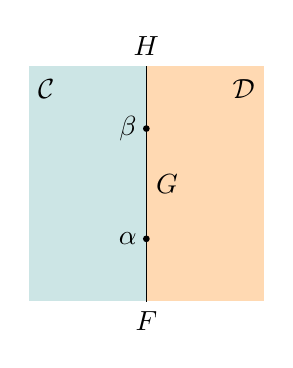
\begin{tikzpicture}
\def\x{0};
\def\xl{-1.5};
\def\xr{1.5};


\def \ya{0};
\def \yb{0.8};
\def \ybb{2.2};
\def \yc{3};
\def \yt {2.7};
\def \ymid {1.5}

\filldraw[fill=blue!50!green!20, draw=white] (\xl, \ya) rectangle (\x, \yc);
\filldraw[fill=orange!30, draw=white] (\x, \ya) rectangle (\xr, \yc);

\node[below] (a) at (\x, \ya) {$F$};
\node(b) at (\x, \yb) {};
\node(bb) at (\x, \ybb) {};
\node [above] (c) at (\x, \yc) {$H$};
\node(m)[right] at (\x, \ymid) {$G$};

\node(l)[right] at (\xl, \yt) {$\mathcal{C}$};
\node(r)[left] at (\xr, \yt) {$\mathcal{D}$};

\filldraw[black] (b) circle (1 pt);
\node [left] at (b) {$\alpha$};
\filldraw[black] (bb) circle (1 pt);
\node [left] at (bb) {$\beta$};

\draw (a)  -- (c);

\end{tikzpicture}
\]
如你所见,你可以通过从下到上扫描弦图来重建原始图表。

再次,在Haskell中,我们将处理三个自函子,以及\hask{beta}在\hask{alpha}之后的垂直组合:
\begin{haskell}
alpha :: forall x. F x -> G x
beta  :: forall x. G x -> H x
\end{haskell}
使用常规函数组合实现:
\begin{haskell}
beta_alpha :: forall x. F x -> H x
beta_alpha = beta . alpha
\end{haskell}

让我们继续自然变换的水平组合:
\[
\begin{tikzcd}[column sep=huge]
\mathcal{C}
  \arrow[bend left=50]{r}[name=U, label=above:$F'$]{}
  \arrow[bend right=50]{r}[name=D, label=below:$F$]{} 
 &
\mathcal{D}
  \arrow[bend left=50]{r}[name=U1, label=above:$G'$]{}
  \arrow[bend right=50]{r}[name=D1, label=below:$G$]{} 
 &
\mathcal{E}
  \arrow[shorten <=10pt,shorten >=10pt,Leftarrow,to path={(U) -- node[label=left:$\alpha$] {} (D)}]{}
  \arrow[shorten <=10pt,shorten >=10pt,Leftarrow,to path={(U1) -- node[label=left:$\beta$] {} (D1)}]{}
\end{tikzcd}
\]
这次我们有三个类别,因此我们将有三个区域。

弦图的底部对应于函子$G \circ F$的组合(按此顺序)。顶部对应于$G' \circ F'$。一个自然变换$\alpha$将$F$连接到$F'$;另一个$\beta$将$G$连接到$G'$。
\[
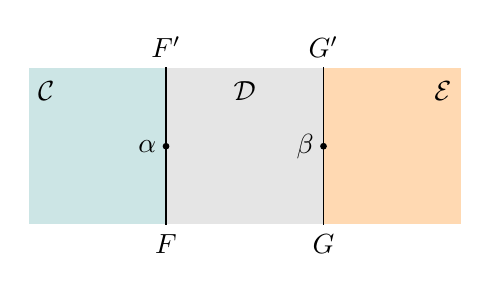
\begin{tikzpicture}
\def\xl{-2.75};
\def\xa{-1};
\def\xc{0}
\def\xb{1};
\def\xr{2.75};


\def \ya{0};
\def \yb{1};
\def \yc{2};
\def \yt {1.7};

\filldraw[fill=blue!50!green!20, draw=white] (\xl, \ya) rectangle (\xa, \yc);
\filldraw[fill=black!10!white, draw=white] (\xa, \ya) rectangle (\xb, \yc);
\filldraw[fill=orange!30, draw=white] (\xb, \ya) rectangle (\xr, \yc);

\node[below] (a) at (\xa, \ya) {$F$};
\node(b) at (\xa, \yb) {};
\node [above] (c) at (\xa, \yc) {$F'$};

\node[below] (d) at (\xb, \ya) {$G$};
\node(e) at (\xb, \yb) {};
\node [above] (f) at (\xb, \yc) {$G'$};

\node(l)[right] at (\xl, \yt) {$\mathcal{C}$};
\node(r) at (\xc, \yt) {$\mathcal{D}$};
\node(r)[left] at (\xr, \yt) {$\mathcal{E}$};


\filldraw[black] (b) circle (1 pt);
\node [left] at (b) {$\alpha$};
\filldraw[black] (e) circle (1 pt);
\node [left] at (e) {$\beta$};

\draw (a)  -- (c);
\draw (d)  -- (f);

\end{tikzpicture}
\]
在这个新系统中,平行的垂直线对应于函子组合。

你可以将自然变换的水平组合视为沿着图表中间的假想水平线发生。但如果有人在绘制图表时粗心,其中一个点比另一个点高一点呢?事实证明,由于交换律,点的确切位置并不重要。

但首先,让我们说明whiskering:其中一个自然变换是恒等变换的水平组合。我们可以这样绘制:

\[
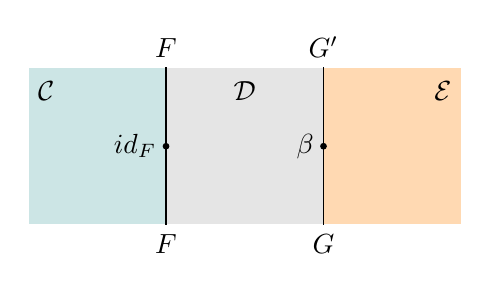
\begin{tikzpicture}
\def\xl{-2.75};
\def\xa{-1};
\def\xc{0}
\def\xb{1};
\def\xr{2.75};


\def \ya{0};
\def \yb{1};
\def \yc{2};
\def \yt {1.7};

\filldraw[fill=blue!50!green!20, draw=white] (\xl, \ya) rectangle (\xa, \yc);
\filldraw[fill=black!10!white, draw=white] (\xa, \ya) rectangle (\xb, \yc);
\filldraw[fill=orange!30, draw=white] (\xb, \ya) rectangle (\xr, \yc);

\node[below] (a) at (\xa, \ya) {$F$};
\node(b) at (\xa, \yb) {};
\node [above] (c) at (\xa, \yc) {$F$};

\node[below] (d) at (\xb, \ya) {$G$};
\node(e) at (\xb, \yb) {};
\node [above] (f) at (\xb, \yc) {$G'$};

\node(l)[right] at (\xl, \yt) {$\mathcal{C}$};
\node(r) at (\xc, \yt) {$\mathcal{D}$};
\node(r)[left] at (\xr, \yt) {$\mathcal{E}$};


\filldraw[black] (b) circle (1 pt);
\node [left] at (b) {$id_F$};
\filldraw[black] (e) circle (1 pt);
\node [left] at (e) {$\beta$};

\draw (a)  -- (c);
\draw (d)  -- (f);

\end{tikzpicture}
\]
但实际上,恒等变换可以插入到垂直线上的任何点,因此我们甚至不需要绘制它。以下图表表示$\beta \circ F$的whiskering。
\[
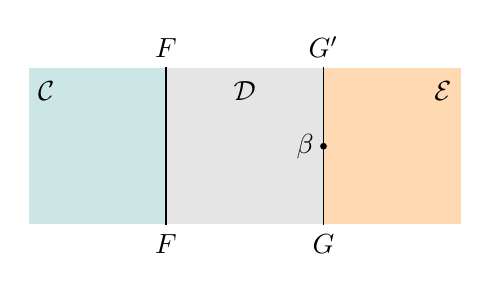
\begin{tikzpicture}
\def\xl{-2.75};
\def\xa{-1};
\def\xc{0}
\def\xb{1};
\def\xr{2.75};


\def \ya{0};
\def \yb{1};
\def \yc{2};
\def \yt {1.7};

\filldraw[fill=blue!50!green!20, draw=white] (\xl, \ya) rectangle (\xa, \yc);
\filldraw[fill=black!10!white, draw=white] (\xa, \ya) rectangle (\xb, \yc);
\filldraw[fill=orange!30, draw=white] (\xb, \ya) rectangle (\xr, \yc);

\node[below] (a) at (\xa, \ya) {$F$};
\node(b) at (\xa, \yb) {};
\node [above] (c) at (\xa, \yc) {$F$};

\node[below] (d) at (\xb, \ya) {$G$};
\node(e) at (\xb, \yb) {};
\node [above] (f) at (\xb, \yc) {$G'$};

\node(l)[right] at (\xl, \yt) {$\mathcal{C}$};
\node(r) at (\xc, \yt) {$\mathcal{D}$};
\node(r)[left] at (\xr, \yt) {$\mathcal{E}$};

\filldraw[black] (e) circle (1 pt);
\node [left] at (e) {$\beta$};

\draw (a)  -- (c);
\draw (d)  -- (f);

\end{tikzpicture}
\]

在Haskell中,其中\hask{beta}是一个多态函数:
\begin{haskell}
beta :: forall x. G x -> G' x
\end{haskell}
我们这样阅读这个图表:
\begin{haskell}
beta_f :: forall x. G (F x) -> G' (F x)
beta_f = beta
\end{haskell}
理解类型检查器为正确类型实例化多态函数\hask{beta}。

同样,你可以轻松想象$G \circ \alpha$的图表及其Haskell实现:
\begin{haskell}
g_alpha :: forall x. G (F x) -> G (F' x)
beta_f = fmap alpha
\end{haskell}
其中:
\begin{haskell}
alpha :: forall x. F x -> F' x
\end{haskell}

这是对应于交换律的弦图:
\[
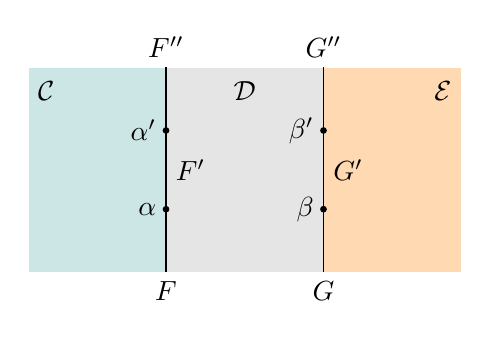
\begin{tikzpicture}
\def\xl{-2.75};
\def\xa{-1};
\def\xc{0}
\def\xb{1};
\def\xr{2.75};


\def \ya{0.2};
\def \yb{1};
\def \ybb{2}
\def \yc{2.8};
\def \yt {\yc -0.3};
\def \ymid {1.5}

\filldraw[fill=blue!50!green!20, draw=white] (\xl, \ya) rectangle (\xa, \yc);
\filldraw[fill=black!10!white, draw=white] (\xa, \ya) rectangle (\xb, \yc);
\filldraw[fill=orange!30, draw=white] (\xb, \ya) rectangle (\xr, \yc);

\node[below] (a) at (\xa, \ya) {$F$};
\node(b) at (\xa, \yb) {};
\node [above] (c) at (\xa, \yc) {$F''$};
\node [right] (ml) at (\xa, \ymid) {$F'$};

\node[below] (d) at (\xb, \ya) {$G$};
\node(e) at (\xb, \yb) {};
\node [above] (f) at (\xb, \yc) {$G''$};
\node [right] (ml) at (\xb, \ymid) {$G'$};

\node(l)[right] at (\xl, \yt) {$\mathcal{C}$};
\node(r) at (\xc, \yt) {$\mathcal{D}$};
\node(r)[left] at (\xr, \yt) {$\mathcal{E}$};


\filldraw[black] (b) circle (1 pt);
\node [left] at (b) {$\alpha$};
\filldraw[black] (e) circle (1 pt);
\node [left] at (e) {$\beta$};

\node(bb) at (\xa, \ybb) {};
\node(ee) at (\xb, \ybb) {};

\filldraw[black] (bb) circle (1 pt);
\node [left] at (bb) {$\alpha'$};
\filldraw[black] (ee) circle (1 pt);
\node [left] at (ee) {$\beta'$};

\draw (a)  -- (c);
\draw (d)  -- (f);

\end{tikzpicture}
\]
这个图表故意模糊。我们是应该先进行自然变换的垂直组合,然后进行水平组合?还是应该将$\beta \circ \alpha$和$\beta' \circ \alpha'$水平组合,然后将结果垂直组合?交换律说这无关紧要:结果是相同的。

现在尝试在这个图表中用恒等变换替换一对自然变换。如果你替换$\alpha'$和$\beta'$,你将得到$\beta \circ \alpha$的水平组合。如果你用恒等自然变换替换$\alpha'$和$\beta$,并将$\beta'$重命名为$\beta$,你将得到$\alpha$相对于$\beta$下移的图表,依此类推。

\[
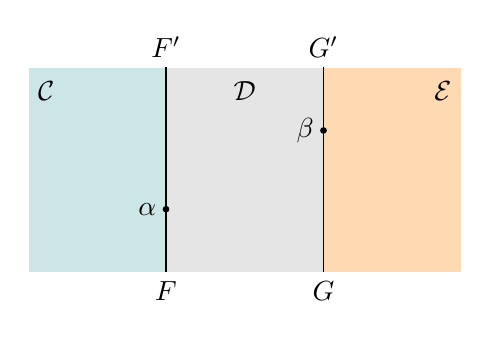
\begin{tikzpicture}
\def\xl{-2.75};
\def\xa{-1};
\def\xc{0}
\def\xb{1};
\def\xr{2.75};


\def \ya{0.2};
\def \yb{1};
\def \ybb{2}
\def \yc{2.8};
\def \yt {\yc -0.3};
\def \ymid {1.5}

\filldraw[fill=blue!50!green!20, draw=white] (\xl, \ya) rectangle (\xa, \yc);
\filldraw[fill=black!10!white, draw=white] (\xa, \ya) rectangle (\xb, \yc);
\filldraw[fill=orange!30, draw=white] (\xb, \ya) rectangle (\xr, \yc);

\node[below] (a) at (\xa, \ya) {$F$};
\node(b) at (\xa, \yb) {};
\node [above] (c) at (\xa, \yc) {$F'$};

\node[below] (d) at (\xb, \ya) {$G$};
\node(e) at (\xb, \yb) {};
\node [above] (f) at (\xb, \yc) {$G'$};

\node(l)[right] at (\xl, \yt) {$\mathcal{C}$};
\node(r) at (\xc, \yt) {$\mathcal{D}$};
\node(r)[left] at (\xr, \yt) {$\mathcal{E}$};


\filldraw[black] (b) circle (1 pt);
\node [left] at (b) {$\alpha$};

\node(bb) at (\xa, \ybb) {};
\node(ee) at (\xb, \ybb) {};

\filldraw[black] (ee) circle (1 pt);
\node [left] at (ee) {$\beta$};

\draw (a)  -- (c);
\draw (d)  -- (f);

\end{tikzpicture}
\]
交换律告诉我们所有这些图表都是相等的。我们可以自由地滑动自然变换,就像在弦上滑动珠子一样。

\subsection{单子的弦图}

单子被定义为一个配备了两个自然变换的自函子,如下面的图表所示:
 
\[
\begin{tikzcd}[column sep=huge]
\mathcal{C}
  \arrow[bend left=50]{r}[name=U, label=above:$T$]{}
  \arrow[bend right=50]{r}[name=D, label=below:$\text{Id}$]{} 
 &
\mathcal{C}
  \arrow[shorten <=10pt,shorten >=10pt,Leftarrow,to path={(U) -- node[label=left:$\eta$] {} (D)}]{}
\end{tikzcd}
\hspace{20pt}
\begin{tikzcd}[column sep=huge]
\mathcal{C}
  \arrow[bend left=50]{r}[name=U, label=above:$T$]{}
  \arrow[bend right=50]{r}[name=D, label=below:$T \circ T$]{} 
 &
\mathcal{C}
  \arrow[shorten <=10pt,shorten >=10pt,Leftarrow,to path={(U) -- node[label=left:$\mu$] {} (D)}]{}
\end{tikzcd}
\]

由于我们只处理一个类别,当将这些图表转换为弦图时,我们可以省略类别的命名(和阴影),只绘制弦。
\[
\begin{tikzpicture}

\def \xleft{-2}

\def\xa{0};
\def\xb{0.7};
\def\xc{\xb * 2};

\def \ya{0};
\def \yb{1};
\def \yc{2};

\node(a) at (\xleft, \ya) {};
\node(b) at (\xleft, \yb) {}; % middle
\node(c) at (\xleft, \yc) {};

\draw[dashed] (a) -- node[right] {$\text{Id}$} (b);
\draw (b) -- node[right] {$T$} (c);


\node(d) at (\xa, \ya) {};
\node(e) at (\xc, \ya) {};
\node(f) at (\xb, \yb) {}; % middle
\node(g) at (\xb, \yc) {}; % top


\filldraw[black] (b) circle (1 pt);
\node [left] at (b) {$\eta$};

\draw (d) to [out=90, in=180]  node[left] {$T$}(f);
\draw (e) to [out=90, in=0]  node[right] {$T$} (f);

\draw (f) -- node[right] {$T$} (g);

\filldraw[black] (f) circle (1 pt);
\node [below] at (f) {$\mu$};

\end{tikzpicture}
\]
在第一个图表中,通常省略对应于恒等函子的虚线。$\eta$点可以自由地将$T$线注入图表中。两条$T$线可以通过$\mu$点连接。

弦图在表达单子定律时特别有用。例如,我们有左单位律:
\[ \mu \circ (\eta \circ T) = id \]
可以可视化为一个交换图表:
\[
 \begin{tikzcd}
 \text{Id} \circ T
 \arrow[rr, "\eta \circ T"]
 \arrow[rrd, "id"']
& & T \circ T
 \arrow[d, "\mu"]
 \\
 && T
  \end{tikzcd}
\]
相应的弦图表示通过这个图表的两个路径的相等性:
\[
\begin{tikzpicture}
\def\xa{0};
\def\xb{0.7};
\def\xc{\xb * 2};

\def \ya{0.8};
\def \yb{1.7};
\def \yc{2.6};

\node(a) at (\xa, \ya) {};
\node(b) at (\xb, \yb) {};
\node(c) at (\xc, 0) {};
\node(d) at (\xb, \yc) {};
\filldraw[black] (a) circle (1 pt);
\node [below] at (a) {$\eta$};
\filldraw[black] (b) circle (1 pt);
\node [below] at (b) {$\mu$};
\draw (a) to [out=90, in=180]  node[left] {$T$}(b);
\draw (c) to [out=90, in=0]  node[right] {$T$} (b);
\draw (b) -- node[right] {$T$} (d);

\def\xd{3.5}
\def\xe{2.5}
\node(e) at (\xd, 0) {};
\node(f) at (\xd, \yc) {};
\node at (\xe, 1.5) {$=$};
\draw (e) -- node[right] {$T$} (f);
\end{tikzpicture}
\]
你可以将这种相等性视为拉紧顶部和底部弦的结果,导致$\eta$附加部分被缩回直线。

有一个对称的右单位律:
\[
\begin{tikzpicture}
\def\xa{0};
\def\xb{0.7};
\def\xc{\xb * 2};

\def \ya{0.8};
\def \yb{1.7};
\def \yc{2.6};

\node(a) at (\xa, 0) {};
\node(b) at (\xb, \yb) {};
\node(c) at (\xc, \ya) {};
\node(d) at (\xb, \yc) {};
\filldraw[black] (b) circle (1 pt);
\node [below] at (c) {$\eta$};
\filldraw[black] (c) circle (1 pt);
\node [below] at (b) {$\mu$};
\draw (a) to [out=90, in=180]  node[left] {$T$}(b);
\draw (c) to [out=90, in=0]  node[right] {$T$} (b);
\draw (b) -- node[right] {$T$} (d);

\def\xd{3.5}
\def\xe{2.5}
\node(e) at (\xd, 0) {};
\node(f) at (\xd, \yc) {};
\node at (\xe, 1.5) {$=$};
\draw (e) -- node[right] {$T$} (f);
\end{tikzpicture}
\]

最后,这是弦图形式的结合律:
\[
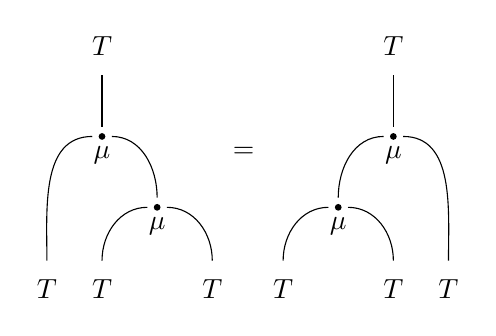
\begin{tikzpicture}
\def\delta{0.7}
\def\xa{0};
\def\xb{\delta};
\def\xc{\delta * 2};
\def\xd{\delta * 3};

\def \ya{0.8};
\def \yb{1.7};
\def \yc{2.6};

\node(a) at (\xa, 0) {};
\node(b) at (\xb, \yb) {};
\node(c) at (\xc, \ya) {};
\node(d) at (\xb, \yc) {};
\node(e) at (\xb, 0) {};
\node(f) at (\xd, 0) {};
\filldraw[black] (b) circle (1 pt);
\filldraw[black] (c) circle (1 pt);
\node [below] at (b) {$\mu$};
\draw (a) to [out=90, in=180]  node[left] {}(b);
\draw (c) to [out=90, in=0]  node[right] {} (b);
\draw (b) -- node[right] {} (d);
\draw (e) to [out=90, in=180]  node[left] {}(c);
\draw (f) to [out=90, in=0]  node[right] {}(c);
\node [below] at (c) {$\mu$};
\node [below] at (a) {$T$};
\node [above] at (d) {$T$};
\node [below] at (e) {$T$};
\node [below] at (f) {$T$};

\def\xe{2.5}
\node at (\xe, 1.5) {$=$};

\def\off{3}
\def\xa{\off + \delta * 0};
\def\xb{\off + \delta * 1};
\def\xc{\off + \delta * 2};
\def\xd{\off + \delta * 3};

\node(a) at (\xa, 0) {};
\node(b) at (\xc, 0) {};
\node(c) at (\xd, 0) {};
\node(d) at (\xb, \ya) {};
\node(e) at (\xc, \yb) {};
\node(f) at (\xc, \yc) {};
\filldraw[black] (d) circle (1 pt);
\filldraw[black] (e) circle (1 pt);
\node [below] at (d) {$\mu$};
\draw (a) to [out=90, in=180]  node[left] {}(d);
\draw (b) to [out=90, in=0]  node[right] {} (d);
\draw (e) -- node[right] {} (f);
\draw (d) to [out=90, in=180]  node[left] {}(e);
\draw (c) to [out=90, in=0]  node[right] {}(e);
\node [below] at (e) {$\mu$};
\node [below] at (a) {$T$};
\node [below] at (b) {$T$};
\node [below] at (c) {$T$};
\node [above] at (f) {$T$};
\end{tikzpicture}
\]

\subsection{伴随的弦图}

正如我们之前讨论的,伴随(adjunction)是一对函子之间的关系,即 $L \colon \mathcal{D} \to \mathcal{C}$ 和 $R \colon \mathcal{C} \to \mathcal{D}$。它可以通过一对自然变换来定义,即单位(unit)$\eta$ 和余单位(counit)$\varepsilon$,它们满足三角恒等式。

伴随的单位可以用一个“杯”形图来表示:

\[
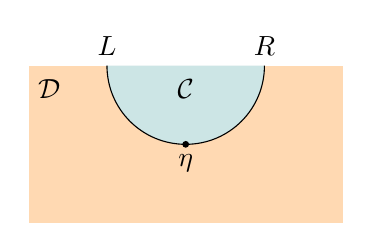
\begin{tikzpicture}

\def \xrightmost {2}
\def \xright         {1}
\def \xmid          {0}
\def \xleft           {-\xright}
\def \xleftmost   {-\xrightmost}

\def \ybot           {0}
\def \ymid          {1}
\def \ytop           {2}
\def \ylabel        {\ytop - 0.3}

% functor labels
\node [above] at (\xleft, \ytop)   {$L$};
\node [above] at (\xright, \ytop) {$R$};
% background
\filldraw[fill=orange!30, draw=white] (\xleftmost, \ytop) rectangle (\xrightmost, \ybot);
% cup
\draw [fill=blue!50!green!20] (\xleft, \ytop) to [out=-90, in=180] (\xmid, \ymid) to [out=0, in=-90] (\xright, \ytop);
% natural transformation
\filldraw [black] (\xmid, \ymid) circle (1 pt);
\node [below] at (\xmid, \ymid) {$\eta$};
% category labels
\node           at (\xmid, \ylabel)        {$\mathcal{C}$};
\node [right] at (\xleftmost, \ylabel) {$\mathcal{D}$};

\end{tikzpicture}
\]
图中底部的恒等函子被省略了。$\eta$ 点将其下方的恒等函子转换为其上方的复合函子 $R \circ L$。

类似地,余单位可以可视化为一个“帽”形弦图,其中顶部的恒等函子是隐含的:

\[
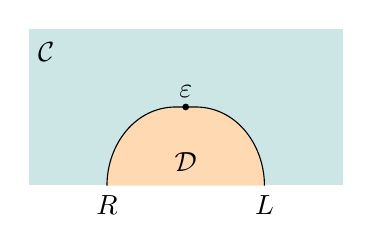
\begin{tikzpicture}
\def\xleft{0};
\def\xmid{1};
\def\xright{\xmid * 2};

\def \ybot{0};
\def \ymid{1};
\def \ytop{2 * \ymid};
\def \yt{2 * \ymid - 0.3};

\node [below] (a) at (\xleft, \ybot) {$R$};
\node(b) at (\xmid, \ymid) {};
\node[below] (c) at (\xright, \ybot) {$L$};

\filldraw[fill=blue!50!green!20, draw=white] (\xleft-1, \ytop) rectangle (\xright+1, \ybot);


\draw [fill=orange!30] (a.north) to [out=90, in=180] (b.west) -- (b.east) to [out=0, in=90] (c.north);

\filldraw[black] (b) circle (1 pt);
\node [above] at (b) {$\varepsilon$};

\node(l)[right] at (\xleft-1, \yt) {$\mathcal{C}$};
\node(r) at (\xmid, \ybot + 0.3) {$\mathcal{D}$};

\end{tikzpicture}
\]

三角恒等式可以很容易地用弦图表示。它们也具有直观的意义,因为你可以想象从两侧拉弦以拉直曲线。

例如,这是第一个三角恒等式,有时称为\index{zigzag identity}\emph{之字形}恒等式:

\[
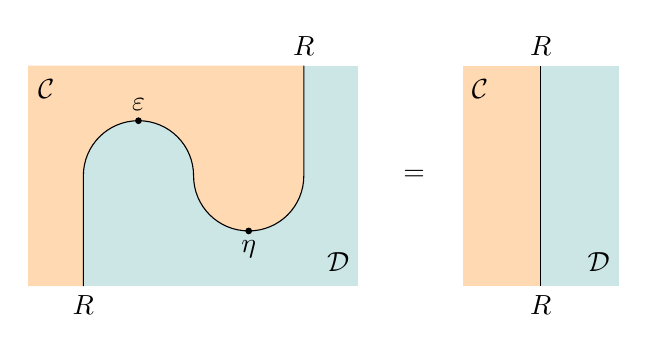
\begin{tikzpicture}
\def \dx {0.7}
\def \dy {0.7}

\def \xa{-3 * \dx};
\def \xb{-2 * \dx};
\def \xc{-1 * \dx};
\def \xd{0};
\def \xe{1 * \dx};
\def \xf{2 * \dx};
\def \xg{3 * \dx};

\def \ya{0};
\def \yb{1 * \dy};
\def \yc{2 * \dy};
\def \yd{3 * \dy};
\def \ye{4 * \dy};

\node [below] at (\xb, \ya) {$R$};
\node [right] at (\xd, \yc) {$L$};
\node [above] at (\xf, \ye) {$R$};
% background
\filldraw[fill=blue!50!green!20, draw=white] (\xa, \ye) rectangle (\xg, \ya);
% fill shape
\path [fill=orange!30] (\xa, \ya) to (\xb, \ya) to (\xb, \yc) to [out=90, in=180]  (\xc, \yd) to  [out=0, in=90] (\xd, \yc) to [out=-90, in=180] (\xe, \yb) to [out=0, in=-90] (\xf, \yc) to (\xf, \ye) to (\xa, \ye);

\draw (\xb, \ya) to (\xb, \yc) to [out=90, in=180]  (\xc, \yd) to  [out=0, in=90] (\xd, \yc) to [out=-90, in=180] (\xe, \yb) to [out=0, in=-90] (\xf, \yc) to (\xf, \ye);

\filldraw[black] (\xc, \yd) circle (1 pt);
\node [above] at (\xc, \yd) {$\varepsilon$};

\filldraw[black] (\xe, \yb) circle (1 pt);
\node [below] at (\xe, \yb) {$\eta$};

\node[right] at (\xa, \ye - 0.3) {$\mathcal{C}$};
\node[left] at (\xg, \ya + 0.3) {$\mathcal{D}$};

% right diagram

\node (eq) at (4 * \dy, \yc) {$=$};
\def \xh {6.3 * \dx}

\filldraw[fill=orange!30, draw=white] (\xh - 1, \ye) rectangle (\xh, \ya);
\filldraw[fill=blue!50!green!20, draw=white] (\xh, \ye) rectangle (\xh + 1, \ya);

\draw (\xh, \ye) -- (\xh, \ya);

\node[below] (bb) at (\xh, \ya) { $R$ };
\node[above] (bt) at (\xh, \ye) { $R$ };

\node(l)[right] at (\xh - 1, \ye - 0.3) {$\mathcal{C}$};
\node(r)[left] at (\xh + 1, \ya + 0.3) {$\mathcal{D}$};

\end{tikzpicture}
\]
从左图自下而上读取,产生一系列映射:

\[  Id_{\mathcal{D}} \circ R \xrightarrow{\eta \circ R} R \circ L \circ R \xrightarrow{R \circ \varepsilon} R \circ Id_{\mathcal{C}}  \]
这必须等于右侧,可以将其解释为 $R$ 上的(隐式的)恒等自然变换。

在 $R$ 是自函子的情况下,我们可以直接将第一个图转换为 Haskell。伴随的单位 $\eta$ 通过 $R$ 的“whiskering”导致多态函数 \hask{unit} 在 \hask{R x} 处实例化。$\varepsilon$ 的“whiskering”导致 \hask{counit} 通过函子 $R$ 的提升。垂直复合转换为函数复合:
\begin{haskell}
triangle :: forall x. R x -> R x
triangle = fmap counit . unit
\end{haskell}

\begin{exercise}
绘制第二个三角恒等式的弦图并将其转换为 Haskell。
\end{exercise}

\section{从伴随函子导出的单子}

你可能已经注意到,相同的符号 $\eta$ 被用于伴随函子的单位(unit)和单子的单位。这 \emph{并非} 巧合。

乍一看,我们似乎是在比较苹果和橘子:伴随函子是由两个范畴之间的两个函子定义的,而单子是由作用于单个范畴的一个自函子(endofunctor)定义的。然而,两个方向相反的函子的复合是一个自函子,而伴随函子的单位将恒等自函子映射到自函子 $R \circ L$。

比较以下图表:
\[
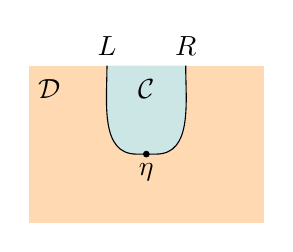
\begin{tikzpicture}
\def\xleft{0.5};
\def\xmid{1};
\def\xright{1.5};

\def \ybot{0};
\def \ymid{1};
\def \ytop{2 * \ymid};
\def \yt{2 * \ymid - 0.3};

\node [above] (a) at (\xleft, \ytop) {$L$};
\node(b) [below] at (\xmid, \ymid) {};
\node[above] (c) at (\xright, \ytop) {$R$};

\filldraw[fill=orange!30, draw=white] (\xleft-1, \ytop) rectangle (\xright+1, \ybot);


\draw [fill=blue!50!green!20] (a.south) to [out=-90, in=180] (b.west) -- (b.east) to [out=0, in=-90] (c.south);
\filldraw[black] (b) circle (1 pt);
\node [below] at (b) {$\eta$};

\node(l)[right] at (\xleft-1, \yt) {$\mathcal{D}$};
\node(r) at (\xmid, \yt) {$\mathcal{C}$};

\end{tikzpicture}
\]
与定义单子单位的图表:

\[
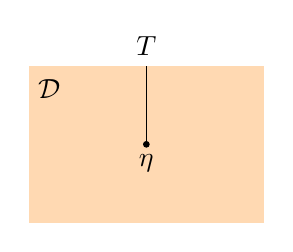
\begin{tikzpicture}
\def\xleft{0.5};
\def\xmid{1};
\def\xright{1.5};

\def \ybot{0};
\def \ymid{1};
\def \ytop{2 * \ymid};
\def \yt{2 * \ymid - 0.3};

\node(b) [above] at (\xmid, \ytop) {$T$};

\filldraw[fill=orange!30, draw=white] (\xleft-1, \ytop) rectangle (\xright+1, \ybot);

\draw (\xmid, \ymid) -- (\xmid, \ytop);

\filldraw[black] (\xmid, \ymid) circle (1 pt);
\node [below] at (\xmid, \ymid) {$\eta$};

\node(l)[right] at (\xleft-1, \yt) {$\mathcal{D}$};

\end{tikzpicture}
\]

事实证明,对于任何伴随函子 $L \dashv R$,自函子 $T = R \circ L$ 都是一个单子,其乘法 $\mu$ 由以下图表定义:

\[
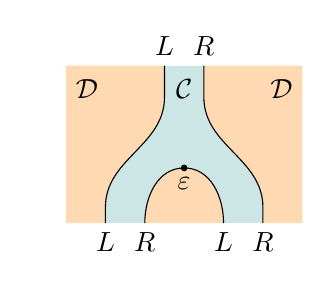
\begin{tikzpicture}
\def \xmid          {0};
\def \xr               {0.5};
\def \xrr             {1}
\def \xrm            {0.25}
\def \xrightmost {1.5}
\def \xl {-\xr}
\def \xll {-\xrr}
\def \xlm {-\xrm}
\def \xleftmost {-\xrightmost}

\def \ybot           {0};
\def \ymidbot     {0.20};
\def \yeps          {0.7};
\def \ymid          {1};
\def \ymidtop     {1.60}
\def \ytop           {2};
\def \ylabel        {\ytop - 0.3};
% functors
\node [above] at (\xlm, \ytop)  {$L$};
\node [above] at (\xrm, \ytop) {$R$};
\node [below] at (\xll, \ybot) {$L$};
\node [below] at (\xl, \ybot) {$R$};
\node [below] at (\xr, \ybot) {$L$};
\node [below] at (\xrr, \ybot) {$R$};

\filldraw[fill=blue!50!green!20, draw=white, draw=white] (\xleftmost, \ytop) rectangle (\xrightmost, \ybot);

% left area
\path [fill=orange!30] (\xleftmost, \ybot) to  (\xll, \ybot) to (\xll, \ymidbot) [out=90, in=-90] to (\xlm, \ymidtop) to  (\xlm, \ytop) to [out=180, in=180] (\xleftmost, \ytop);
% right area
\path [fill=orange!30] (\xrightmost, \ybot) to (\xrr, \ybot) to (\xrr, \ymidbot) [out=90, in=-90] to (\xrm, \ymidtop) to (\xrm, \ytop) to [out=0, in=180]  (\xrightmost, \ytop);
% cap
\draw [fill=orange!30] (\xl, \ybot) to [out=90, in=180] (\xmid, \yeps) to [out=0, in=90] (\xr, \ybot);
% left curve
\draw (\xll, \ybot) to (\xll, \ymidbot) [out=90, in=-90] to (\xlm, \ymidtop) to  (\xlm, \ytop);
% right curve
\draw (\xrr, \ybot) to (\xrr, \ymidbot) [out=90, in=-90] to (\xrm, \ymidtop) to (\xrm, \ytop);
% epsilon
\filldraw [black] (\xmid, \yeps) circle (1 pt);
\node [below] at (\xmid, \yeps) {$\varepsilon$};
% categories
\node [right] at (\xleftmost, \ylabel) {$\mathcal{D}$};
\node           at (\xmid, \ylabel)        {$\mathcal{C}$};
\node [left]   at (\xrightmost, \ylabel) {$\mathcal{D}$};

\end{tikzpicture}
\]
从下到上阅读此图表,我们得到以下变换(想象在点处水平切割):
\[  R \circ L \circ R \circ L \xrightarrow{R \circ \varepsilon \circ L} R \circ L  \]
将其与单子 $\mu$ 的定义进行比较:

\[
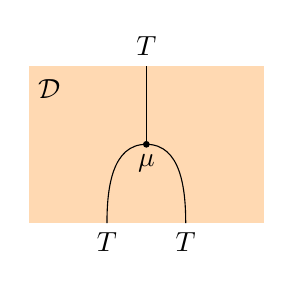
\begin{tikzpicture}
\def \xmid          {0};
\def \xr               {0.5};
\def \xrightmost {1.5};
\def \xl {-\xr};
\def \xleftmost {-\xrightmost};

\def \ybot           {0};
\def \ymid          {1};
\def \ytop           {2};
\def \ylabel        {\ytop - 0.3};

\node [above] at (\xmid, \ytop) {$T$};
\node [below] at (\xl, \ybot)      {$T$};
\node [below] at (\xr, \ybot)      {$T$};

\filldraw[fill=orange!30, draw=white] (\xleftmost, \ytop) rectangle (\xrightmost, \ybot);
% cap
\draw (\xl, \ybot) to [out=90, in=180] (\xmid, \ymid) to [out=0, in=90] (\xr, \ybot);
\draw (\xmid, \ymid) to (\xmid, \ytop);

\filldraw [black] (\xmid, \ymid) circle (1 pt);
\node [below] at (\xmid, \ymid) {$\mu$};

\node [right] at (\xleftmost, \ylabel) {$\mathcal{D}$};

\end{tikzpicture}
\]
我们得到单子 $R \circ L$ 的 $\mu$ 定义为 $\varepsilon$ 的双重whiskering:
\[ \mu = R \circ \varepsilon \circ L \]

在Haskell中,用 $\varepsilon$ 定义 $\mu$ 的字符串图表的翻译总是可能的。单子的乘法,即 \hask{join},变为:
\begin{haskell}
join :: forall x. T (T x) -> T x
join = fmap counit
\end{haskell}
其中 \hask{fmap} 对应于由自函子 \hask{T} 定义的提升,该自函子定义为 $R \circ L$ 的复合。注意,在这种情况下,$\cat D$ 是Haskell的类型和函数的范畴,但 $\cat C$ 可以是一个外部范畴。

为了完善这一图景,我们可以使用字符串图表来推导单子定律,利用三角恒等式。技巧是将单子定律中的所有字符串替换为平行的字符串对,然后根据规则重新排列它们。

总结一下,每个伴随函子 $L \dashv R$ 与单位 $\eta$ 和余单位 $\varepsilon$ 一起定义了一个单子 $(R \circ L, \eta, R \circ \varepsilon \circ L)$。

我们稍后会看到,对偶地,另一种复合 $L \circ R$ 定义了一个余单子(comonad)。

\begin{exercise}
绘制字符串图表来说明从伴随函子导出的单子的单子定律(单位和结合性)。
\end{exercise}

\section{伴随函子生成的单子示例}

我们将通过几个伴随函子的例子,这些伴随函子生成了我们在编程中使用的一些单子。当我们讨论单子变换器时,我们会进一步扩展这些例子。

大多数例子涉及离开Haskell类型和函数范畴的函子,尽管生成单子的往返最终是一个自函子。这就是为什么在Haskell中通常无法表达这样的伴随函子。

此外,由于与数据构造函数的显式命名相关的许多簿记工作,这可能会使底层公式的简洁性变得模糊,而这些簿记工作对于类型推断是必要的。

\subsection{自由幺半群与列表单子}
列表单子是由我们之前见过的自由幺半群伴随函子生成的。这个伴随函子的单位$\eta_X \colon X \to U (F X)$将集合$X$的元素注入为自由幺半群$F X$的生成元,之后$U$提取底层集合。

在Haskell中,我们将自由幺半群表示为列表类型,其生成元是单元素列表。单位$\eta_X$将$X$的元素映射到这样的单元素列表:
\begin{haskell}
return x = [x]
\end{haskell}
为了实现余单位$\varepsilon_M \colon F (U M) \to M$,我们取一个幺半群$M$,忘记其乘法,并使用其元素集合作为新自由幺半群的生成元。$M$处的余单位分量是从自由幺半群回到$M$的幺半群态射,或者在Haskell中为\hask{[m]->m}。事实证明,这个幺半群态射是catamorphism的一个特例。

首先,回忆一下Haskell中一般列表catamorphism的实现:
\begin{haskell}
foldMap :: Monoid m => (a -> m) -> ([a] -> m)
foldMap f = foldr mappend mempty . fmap f
\end{haskell}
在这里,我们将\hask{(a -> m)}解释为从\hask{a}到幺半群\hask{m}的底层集合的常规函数。结果被解释为从由\hask{a}生成的自由幺半群(即\hask{a}的列表)到\hask{m}的\emph{幺半群态射}。这只是伴随函子的一个方向:
\[ \Set (a, U m) \cong \Cat{Mon} (F a, m) \]

为了将余单位作为幺半群态射\hask{[m]->m},我们将\hask{foldMap}应用于恒等函数。结果是\hask{(foldMap id)},或者用\hask{foldr}表示:
\begin{haskell}
epsilon = foldr mappend mempty
\end{haskell}
它是一个幺半群态射,因为它将空列表映射到幺半群单位,并将连接映射到幺半群积。

单子乘法,或\hask{join},由余单位的whiskering给出:
\[ \mu = U \circ \varepsilon \circ F \]
你可以很容易地相信,这里的左whiskering并没有做太多事情,因为它只是通过遗忘函子提升了一个幺半群态射(它保留了函数,同时忘记了其保持结构的特殊性质)。

由$F$进行的右whiskering更有趣。这意味着分量$\mu_X$对应于$F X$处的$\varepsilon$分量,即由集合$X$生成的自由幺半群。这个自由幺半群定义为:
\begin{haskell}
mempty = []
mappend = (++)
\end{haskell}
这给出了\hask{join}的定义:
\begin{haskell}
join = foldr (++) []
\end{haskell}
正如预期的那样,这与\hask{concat}相同:在列表单子中,乘法是连接。

\subsection{柯里化伴随函子与状态单子}

状态单子是由我们用来定义指数对象的柯里化伴随函子生成的。左函子由与某个固定对象$s$的积定义:
\[ L_s a = a \times s \]
例如,我们可以将其实现为Haskell类型:
\begin{haskell}
newtype L s a = L (a, s)
\end{haskell}
右函子是指数,由相同的对象$s$参数化:
\[ R_s c = c^s \]
在Haskell中,它是一个薄封装的函数类型:
\begin{haskell}
newtype R s c = R (s -> c)
\end{haskell}

单子由这两个函子的组合给出。在对象上:
\[(R_s \circ L_s) a = (a \times s)^s \]
在Haskell中,我们可以将其写为:
\begin{haskell}
newtype St s a = St (R s (L s a))
\end{haskell}
如果你展开这个定义,很容易在其中识别出\hask{State}函子:
\begin{haskell}
newtype State s a = State (s -> (a, s))
\end{haskell}

伴随函子$L_s \dashv R_s$的单位是一个映射:
\[ \eta_a \colon a \to (a \times s)^s \]
可以在Haskell中实现为:
\begin{haskell}
unit :: a -> R s (L s a)
unit a = R (\s -> L (a, s))
\end{haskell}
你可能会在其中识别出状态单子的\hask{return}的薄封装版本:
\begin{haskell}
return :: a -> State s a
return a = State (\s -> (a, s))
\end{haskell}

这是$c$处这个伴随函子的余单位分量:
\[ \varepsilon_c \colon c^s \times s \to c \]
可以在Haskell中实现为:
\begin{haskell}
counit :: L s (R s a) -> a
counit (L ((R f), s))= f s
\end{haskell}
在剥离数据构造函数后,这等同于\hask{apply},或\hask{runState}的非柯里化版本。

单子乘法$\mu$由$\varepsilon$的whiskering给出:
\[ \mu = R_s \circ \varepsilon \circ L_s \]
这是它在Haskell中的翻译:
\begin{haskell}
mu :: R s (L s (R s (L s a))) -> R s (L s a)
mu = fmap counit
\end{haskell}
右whiskering除了选择自然变换的分量外,没有做任何事情。这是由Haskell的类型推断引擎自动完成的。左whiskering通过提升自然变换的分量来完成。再次,类型推断选择了正确的\hask{fmap}实现——在这里,它等同于预组合。

将其与\hask{join}的实现进行比较:
\begin{haskell}
join :: State s (State s a) -> State s a
join mma = State (fmap (uncurry runState) (runState mma))
\end{haskell}
注意\hask{runState}的双重使用:
\begin{haskell}
runState :: State s a -> s -> (a, s)
runState (State h) s = h s
\end{haskell}
当它被非柯里化时,其类型签名变为:
\begin{haskell}
uncurry runState :: (State s a, s) -> (a, s)
\end{haskell}
这等同于\hask{counit}的类型签名。

当部分应用时,\hask{runState}只是剥离数据构造函数,暴露底层函数类型:
\begin{haskell}
runState st :: s -> (a, s)
\end{haskell}

\subsection{M-集与Writer单子}

Writer单子:
\begin{haskell}
newtype Writer m a = Writer (a, m)
\end{haskell}
由一个幺半群\hask{m}参数化。这个幺半群用于累积日志条目。我们将使用的伴随函子涉及该幺半群的M-集范畴。

一个\index{M-集}M-集是一个集合$S$,我们在其上定义了一个幺半群$M$的作用。这样的作用是一个映射:
\[a \colon M \times S \to S \]
我们经常使用作用的柯里化版本,将幺半群元素放在下标位置。因此$a_m$成为一个函数$S \to S$。

这个映射必须满足一些约束。幺半群单位$1$的作用不能改变集合,因此它必须是恒等函数:
\[ a_1 = id_S \]
并且两个连续的作用必须组合成它们的幺半群积的作用:
\[ a_{m_1} \circ a_{m_2} = a_{m_1 \cdot m_2} \]
这种乘法顺序的选择定义了所谓的\emph{左作用}。(右作用将两个幺半群元素在右侧交换。)

M-集形成一个范畴$\mathbf{MSet}$。对象是$(S, a\colon M\times S \to S)$,箭头是\index{等变映射}\emph{等变映射},即保持作用的集合之间的函数。

一个函数$f \colon S \to R$是从$(S, a)$到$(R, b)$的\emph{等变}映射,如果对于每个$m \in M$,以下图表交换:

\[
 \begin{tikzcd}
 S 
 \arrow[r, "f"]
 \arrow[d, "a_m"]
 & R
\arrow[d, "b_m"]
 \\
S
 \arrow[r, "f"]
 & R
  \end{tikzcd}
\]
换句话说,无论我们是先做作用$a_m$,然后映射集合;还是先映射集合,然后做相应的作用$b_m$,结果都是一样的。

有一个遗忘函子$U$从$\mathbf{MSet}$到$\mathbf{Set}$,它将集合$S$分配给对$(S, a)$,从而忘记作用。

与之对应的是一个自由函子$F$。它对集合$S$的作用产生一个M-集。它是一个集合,是$S$和$M$的笛卡尔积,其中$M$被视为元素集合(换句话说,遗忘函子对幺半群作用的结果)。这个M-集的一个元素是$(x \in S, m \in M)$,自由作用定义为:
\[ \phi_n \colon (x, m) \mapsto (x, n \cdot m) \]
保持元素$x$不变,只乘以$m$分量。

为了证明$F$是$U$的左伴随函子,我们必须构造以下自然同构:
\[ \mathbf{MSet}( F S, Q) \cong \mathbf{Set}(S, U Q) \]
对于任何集合$S$和任何M-集$Q$。如果我们将$Q$表示为$(R, b)$,伴随函子右侧的元素是一个普通函数$u \colon S \to R$。我们可以使用这个函数在左侧构造一个等变映射。

这里的技巧是注意到这样的等变映射$f \colon F S \to Q$完全由其在形式为$(x, 1) \in F S$的元素上的作用决定,其中$1$是幺半群单位。

实际上,从等变条件可以得出:
\[
 \begin{tikzcd}
 (x, 1)
 \arrow[r, mapsto, "f"]
 \arrow[d, mapsto, "\phi_m"]
 & r
\arrow[d, mapsto, "b_m"]
 \\
(x, m \cdot 1)
 \arrow[r, mapsto, "f"]
 & r'
  \end{tikzcd}
\]
或者:
\[ f( \phi_m (x, 1)) = f (x, m) = b_m ( f (x, 1)) \]
因此,每个函数$u \colon S \to R$唯一地定义了一个等变映射$f \colon F S \to Q$,由下式给出:
\[ f (x, m) = b_m (u x) \]

这个伴随函子的单位$\eta_S \colon S \to U (F S)$将一个元素$x$映射到对$(x, 1)$。将其与Writer单子的\hask{return}定义进行比较:
\begin{haskell}
return a = Writer (a, mempty)
\end{haskell}

余单位由一个等变映射给出:
\[ \varepsilon_Q \colon F (U Q) \to Q \]

左侧是通过取$Q$的底层集合并将其与$M$的底层集合的乘积构造的M-集。$Q$的原始作用被遗忘,并被自由作用取代。余单位的明显选择是:
\[ \varepsilon_Q \colon (x, m) \mapsto a_m x \]
其中$x$是$Q$的(底层集合的)元素,$a$是$Q$中定义的作用。

单子乘法$\mu$由余单位的whiskering给出。
\[ \mu = U \circ \varepsilon \circ F \]
这意味着在$\varepsilon_Q$的定义中用自由M-集替换$Q$,其作用是自由作用。换句话说,我们用$(x, m)$替换$x$,用$\phi_n$替换$a_n$。(与$U$的whiskering没有改变任何东西。)
\[ \mu_S \colon ((x, m), n) \mapsto \phi_n (x, m) = (x, n \cdot m) \]
将其与Writer单子的\hask{join}定义进行比较:
\begin{haskell}
join :: Monoid m => Writer m (Writer m a) -> Writer m a
join (Writer ( Writer (x, m), n)) = Writer (x, mappend n m)
\end{haskell}

\subsection{点对象与\hask{Maybe}单子}

点对象是具有指定元素的对象。由于选择元素是使用从终端对象的箭头完成的,点对象的范畴使用对$(a, p \colon 1 \to a)$定义,其中$a$是$\mathcal{C}$中的对象。

这些对之间的态射是$\mathcal{C}$中保持点的箭头。因此,从$(a, p \colon 1 \to a)$到$(b, q \colon 1 \to b)$的态射是一个箭头$f \colon a \to b$,使得$q = f \circ p$。这个范畴也被称为\index{余切片}\emph{余切片范畴},并写为$1/\mathcal{C}$。

有一个明显的遗忘函子$U \colon 1/\mathcal{C} \to \mathcal{C}$,它忘记了点。它的左伴随函子是一个自由函子$F$,它将对象$a$映射到对$(1 + a, \text{Left})$。换句话说,$F$使用余积自由地向对象添加一个点。

\hask{Either}单子类似地通过用固定对象$e$替换$1$来构造。

\begin{exercise}
证明$U \circ F$是\hask{Maybe}单子。
\end{exercise}

\subsection{延续单子}

延续单子是根据集合范畴中的一对逆变函子定义的。我们不需要修改伴随函子的定义来处理逆变函子。只需为其中一个端点选择相反范畴即可。

我们将左函子定义为:
\[ L_Z \colon \mathbf{Set}^{op} \to \mathbf{Set} \] 
它将集合$X$映射到$\mathbf{Set}$中的hom-集:
\[ L_Z X = \mathbf{Set}(X, Z) \] 
这个函子由另一个集合$Z$参数化。右函子由基本相同的公式定义:
\[ R_Z \colon \mathbf{Set} \to \mathbf{Set}^{op} \] 
\[ R_Z X = \mathbf{Set^{op}}(Z, X)  = \mathbf{Set}(X, Z) \] 

组合$R \circ L$可以在Haskell中写为\hask{((x -> r) -> r)},这与定义延续单子的(协变)自函子相同。

\section{单子变换器(Monad Transformers)}

假设你想组合多个效应,例如状态与可能的失败。一种选择是从头定义你自己的单子。你定义一个函子:
\begin{haskell}
newtype MaybeState s a = MS (s -> Maybe (a, s))
  deriving Functor
\end{haskell}
同时定义提取结果(或报告失败)的函数:
\begin{haskell}
runMaybeState :: MaybeState s a -> s -> Maybe (a, s)
runMaybeState (MS h) s = h s
\end{haskell}
你为它定义单子实例:
\begin{haskell}
instance Monad (MaybeState s) where
  return a = MS (\s -> Just (a, s))
  ms >>= k = MS (\s -> case runMaybeState ms s of
                       Nothing -> Nothing
                       Just (a, s') -> runMaybeState (k a) s')
\end{haskell}
并且,如果你足够勤奋,检查它是否满足单子定律。

没有通用的方法来组合单子。从这个意义上说,单子是不可组合的。然而,我们知道伴随(adjunctions)是可组合的。我们也已经看到如何从伴随中获取单子,并且,正如我们将要看到的,每个单子都可以通过这种方式获得。因此,如果我们能匹配伴随,它们生成的单子将自动组合。

考虑两个可组合的伴随:
\[
 \begin{tikzcd}
  \mathcal{C}
  \arrow[rr, bend right, "R'"']
  &&
  \mathcal{D}
  \arrow[ll, bend right, "L'"']
    \arrow[rr, bend right, "R"']
&&
  \mathcal{E}
  \arrow[ll, bend right, "L"']
 \end{tikzcd}
\]
这幅图中有三个单子。有“内部”单子 $R' \circ L'$ 和“外部”单子 $R \circ L$ 以及组合 $R \circ R' \circ L' \circ L$。

如果我们称内部单子为 $T = R' \circ L'$,那么 $R \circ T \circ L$ 就是组合单子,称为\emph{单子变换器},因为它将单子 $T$ 转换为一个新的单子。

\[
 \begin{tikzcd}
   &&
  \mathcal{D}
  \arrow[loop, "T = R' \circ L'"']
    \arrow[rr, bend right, "R"']
&&
  \mathcal{E}
  \arrow[ll, bend right, "L"']
 \end{tikzcd}
\]

在我们的例子中,我们可以将 \hask{Maybe} 视为内部单子:
\[ T a = 1 + a \]
它使用生成状态单子的外部伴随 $L_s \dashv R_s$ 进行变换:
\[ L_s a = a \times s \]
\[ R_s c = c^s \]
结果是:
\[ (R_s \circ T \circ L_s) a = (1 + a \times s)^s\]
或者,在 Haskell 中:
\begin{haskell}
s -> Maybe (a, s)
\end{haskell}
这与我们的 \hask{MaybeState} 单子的定义一致。

一般来说,内部单子 $T$ 由其单位 $\eta^i$ 和乘法 $\mu^i$ 定义(上标 $i$ 表示“内部”)。外部伴随由其单位 $\eta^o$ 和余单位 $\varepsilon^o$ 定义。

组合单子的单位是自然变换:
\[ \eta \colon Id \to R \circ T \circ L \]
由字符串图给出:
\[
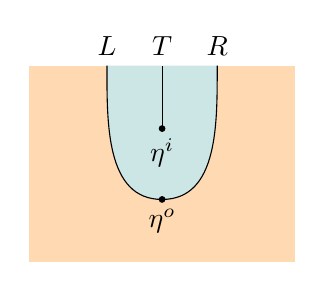
\begin{tikzpicture}
\def\xright{0.7};
\def\xleft{-\xright};
\def\xmid{0};

\def \ybot{0};
\def \ymid{0.8};
\def \yup{1.7};
\def \ytop{2.5};

\node [above] at (\xleft, \ytop) {$L$};
\node [above] at (\xmid, \ytop) {$T$};
\node [above] at (\xright, \ytop) {$R$};

\filldraw[fill=orange!30, draw=white] (\xleft-1, \ytop) rectangle (\xright+1, \ybot);

\draw [fill=blue!50!green!20] (\xleft, \ytop) to [out=-90, in=180] (\xmid, \ymid) to [out=0, in=-90] (\xright, \ytop);

\filldraw[black] (\xmid, \ymid) circle (1 pt);
\node [below] at (\xmid, \ymid) {$\eta^o$};
\filldraw[black] (\xmid, \yup) circle (1 pt);
\node [below] at (\xmid, \yup) {$\eta^i$};
\draw (\xmid, \yup) -- (\xmid,\ytop);

\end{tikzpicture}
\]
它是内部单位 $R \circ \eta^i \circ L$ 和外部单位 $\eta^o$ 的垂直组合。在分量中:
\[ \eta_a = R(\eta^i_{L a}) \circ \eta^o_a\]

组合单子的乘法是一个自然变换:
\[ \mu \colon R \circ T \circ L \circ R \circ T \circ L \to R \circ T \circ L \]
由字符串图给出:

\[
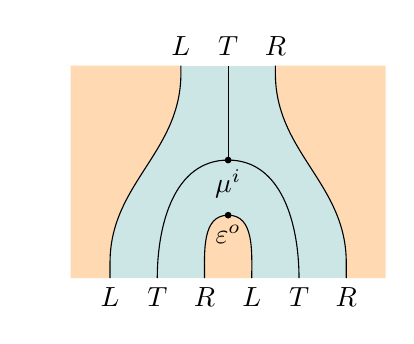
\begin{tikzpicture}
\def \xmid          {0};
\def \xr               {0.3};
\def \xrt             {0.9};
\def \xrr             {1.5}
\def \xrm            {0.6}
\def \xrightmost {2}
\def \xl {-\xr}
\def \xlt {-\xrt}
\def \xll {-\xrr}
\def \xlm {-\xrm}
\def \xleftmost {-\xrightmost}

\def \ybot           {0};
\def \ymidbot     {0.2};
\def \yeps          {0.8};
\def \ymu           {1.5}; % mu
\def \ymid          {1.9};
\def \ymidtop     {2.6}
\def \ytop           {2.7};
\def \ylabel        {\ytop - 0.3};
% functors
\node [above] at (\xlm, \ytop)  {$L$};
\node [above] at (\xmid, \ytop)  {$T$};
\node [above] at (\xrm, \ytop) {$R$};

\node [below] at (\xll, \ybot) {$L$};
\node [below] at (\xlt, \ybot) {$T$};
\node [below] at (\xl, \ybot) {$R$};
\node [below] at (\xr, \ybot) {$L$};
\node [below] at (\xrt, \ybot) {$T$};
\node [below] at (\xrr, \ybot) {$R$};

\filldraw[fill=blue!50!green!20, draw=white, draw=white] (\xleftmost, \ytop) rectangle (\xrightmost, \ybot);

% left area
\path [fill=orange!30] (\xleftmost, \ybot) to  (\xll, \ybot) to (\xll, \ymidbot) [out=90, in=-90] to (\xlm, \ymidtop) to  (\xlm, \ytop) to [out=180, in=180] (\xleftmost, \ytop);
% right area
\path [fill=orange!30] (\xrightmost, \ybot) to (\xrr, \ybot) to (\xrr, \ymidbot) [out=90, in=-90] to (\xrm, \ymidtop) to (\xrm, \ytop) to [out=0, in=180]  (\xrightmost, \ytop);
% cap
\draw [fill=orange!30] (\xl, \ybot) to [out=90, in=180] (\xmid, \yeps) to [out=0, in=90] (\xr, \ybot);
% fork
\draw (\xlt, \ybot) to [out=90, in=180] (\xmid, \ymu) to [out=0, in=90] (\xrt, \ybot);

% left curve
\draw (\xll, \ybot) to (\xll, \ymidbot) [out=90, in=-90] to (\xlm, \ymidtop) to  (\xlm, \ytop);
% right curve
\draw (\xrr, \ybot) to (\xrr, \ymidbot) [out=90, in=-90] to (\xrm, \ymidtop) to (\xrm, \ytop);
% epsilon
\filldraw [black] (\xmid, \yeps) circle (1 pt);
\node [below] at (\xmid, \yeps) {$\varepsilon^o$};

% mu
\filldraw [black] (\xmid, \ymu) circle (1 pt);
\node [below] at (\xmid, \ymu) {$\mu^i$};
\draw (\xmid, \ymu) -- (\xmid, \ytop);

\end{tikzpicture}
\]
它是外部余单位的多次whiskered垂直组合:
\[ R \circ T \circ \varepsilon^o \circ T \circ L \]
后跟内部乘法的whiskered $R \circ \mu^i \circ L$。在分量中:
\[ \mu_c = R(\mu^i_{L c}) \circ (R \circ T) (\varepsilon^o_{(T\circ L)c})\]

\subsection{状态单子变换器}

让我们为状态单子变换器的情况展开这些方程。状态单子由柯里化伴随生成。左函子 $L_s$ 是积函子 \hask{(a, s)},右函子 $R_s$ 是指数函子,也称为读者函子 \hask{(s -> a)}。

正如我们之前所见,外部余单位 $\varepsilon^o_a$ 是函数应用:
\begin{haskell}
counit :: (s -> a, s) -> a
counit (f, x) = f x
\end{haskell}
单位 $\eta^o_a$ 是柯里化的对构造函数:
\begin{haskell}
unit :: a -> s -> (a, s)
unit x = \s -> (x, s)
\end{haskell}

我们将保持内部单子 $(T, \eta^i, \mu^i)$ 为任意。在 Haskell 中,我们将这个三元组称为 \hask{m}、\hask{return} 和 \hask{join}。

通过将状态单子变换器应用于单子 $T$ 得到的组合单子是组合 $R \circ T \circ L$,或者在 Haskell 中:
\begin{haskell}
newtype StateT s m a = StateT (s -> m (a, s))
\end{haskell}

\begin{haskell}
runStateT :: StateT s m a -> s -> m (a, s)
runStateT (StateT h) s = h s
\end{haskell}

单子变换器的单位是 $\eta^o$ 和 $R \circ \eta^i \circ L$ 的垂直组合。在分量中:
\[ \eta_a = R(\eta^i_{L a}) \circ \eta^o_a \]

这个公式中有很多移动的部分,所以让我们逐步分析它。我们从右边开始:我们有伴随单位的 $a$ 分量,它是一个从 $a$ 到 $R (L a)$ 的箭头。在 Haskell 中,它是函数 \hask{unit}。
\begin{haskell}
unit :: a -> s -> (a, s)
\end{haskell}
让我们在某个 \hask{x :: a} 处评估这个函数。结果是另一个函数 \hask{s -> (a, s)}。我们将这个函数作为参数传递给 $R(\eta^i_{L a})$。

$\eta^i_{L a}$ 是内部单子的 \hask{return} 在 $L a$ 处的分量。这里,$L a$ 是类型 \hask{(a, s)}。因此,我们将多态函数 \hask{return :: a -> m a} 实例化为函数 \hask{(a, s) -> m (a, s)}。(类型推断器会自动为我们完成此操作。)

接下来,我们使用 $R$ 提升 \hask{return} 的这个分量。这里,$R$ 是指数 $(-)^s$,因此它通过后组合提升函数。它将 \hask{return} 后组合到传递给它的任何函数。在我们的例子中,这是由 \hask{unit} 生成的函数。注意类型匹配:我们将 \hask{(a, s) -> m (a, s)} 后组合到 \hask{s -> (a, s)} 之后。

我们可以将这个组合的结果写为:
\begin{haskell}
return x = StateT (return . \s -> (x, s))
\end{haskell}
或者,内联函数组合:
\begin{haskell}
return x = StateT (\s -> return (x, s))
\end{haskell}
我们插入了数据构造函数 \hask{StateT} 以使类型检查器满意。这是组合单子的 \hask{return},用内部单子的 \hask{return} 表示。

同样的推理可以应用于组合 $\mu$ 在某个 $a$ 处的分量的公式:

\[ \mu_a = R(\mu^i_{L a}) \circ (R \circ T) (\varepsilon^o_{(T\circ L) a})\]
内部 $\mu^i$ 是单子 \hask{m} 的 \hask{join}。应用 $R$ 将其转换为后组合。

外部 $\varepsilon^o$ 是在 $T(L a)$ 或 \hask{m (a, s)} 处取函数应用。它是一个类型为:
\begin{haskell}
(s -> m (a, s), s) -> m (a, s)
\end{haskell}
的函数,插入适当的数据构造函数后,可以写为 \hask{uncurry runStateT}:
\begin{haskell}
uncurry runStateT :: (StateT s m a, s) -> m (a, s)
\end{haskell}
$(R \circ T)$ 的应用使用函子 $R$ 和 $T$ 的组合提升 $\varepsilon$ 的这个分量。前者实现为后组合,后者是单子 \hask{m} 的 \hask{fmap}。

将所有这些放在一起,我们得到了状态单子变换器的 \hask{join} 的无点公式:
\begin{haskell}
join :: StateT s m (StateT s m a) -> StateT s m a
join mma = StateT (join . fmap (uncurry runStateT) . runStateT mma)
\end{haskell}
这里,部分应用的 \hask{(runStateT mma)} 从参数 \hask{mma} 中剥离数据构造函数:
\begin{haskell}
runStateT mma :: s -> m (a, x)
\end{haskell}

我们之前的 \hask{MaybeState} 示例现在可以使用单子变换器重写:
\begin{haskell}
type MaybeState s a = StateT s Maybe a
\end{haskell}

通过将 \hask{StateT} 单子变换器应用于恒等函子,可以恢复原始的 \hask{State} 单子,该函子在库中定义了 \hask{Monad} 实例(注意在此定义中跳过了最后一个类型变量 \hask{a}):
\begin{haskell}
type State s = StateT s Identity
\end{haskell}

其他单子变换器遵循相同的模式。它们在单子变换器库 \hask{MTL} 中定义。

\section{单子代数}

每个伴随都会生成一个单子,到目前为止,我们已经能够为我们感兴趣的所有单子定义伴随。但是,是否每个单子都是由伴随生成的呢?答案是肯定的,并且通常每个单子都有许多伴随——实际上是一个完整的伴随范畴。

为单子找到伴随类似于因式分解。我们希望将一个函子表示为另外两个函子的复合,即 $T = R \circ L$。问题的复杂性在于,这种因式分解还需要找到适当的中间范畴。我们将通过研究单子的代数来找到这样的范畴。

单子由一个自函子定义,我们知道可以为自函子定义代数。数学家通常将单子视为生成表达式的工具,而代数则是评估这些表达式的工具。然而,由单子生成的表达式对这些代数施加了一些兼容性条件。

例如,你可能会注意到单子单位 $\eta_a \colon a \to T a$ 的类型签名看起来像代数结构映射 $\alpha \colon T a \to a$ 的逆。当然,$\eta$ 是一个为每个类型定义的自然变换,而代数有一个固定的载体类型。尽管如此,我们可能会合理地期望其中一个可以抵消另一个的作用。

考虑之前的表达式单子 \hask{Ex} 的例子。这个单子的代数是一个载体类型的选择,比如 \hask{Char} 和一个箭头:
\begin{haskell}
alg :: Ex Char -> Char
\end{haskell}
由于 \hask{Ex} 是一个单子,它定义了一个单位,即 \hask{return},这是一个多态函数,可以用来从值生成简单的表达式。\hask{Ex} 的单位是:
\begin{haskell}
return x = Var x
\end{haskell}
我们可以为任意类型实例化单位,特别是为我们的代数的载体类型。要求 \emph{评估} \hask{Var c}(其中 \hask{c} 是一个字符)应该返回相同的 \hask{c} 是合理的。换句话说,我们希望:
\begin{haskell}
 alg . return = id
\end{haskell}
这个条件将立即排除许多代数,例如:
\begin{haskell}
alg (Var c) = 'a' -- 与单子 Ex 不兼容
\end{haskell}

我们希望施加的第二个条件是,与单子兼容的代数尊重替换。单子允许我们使用 \hask{join} 来展平嵌套表达式。代数允许我们评估这些表达式。

有两种方法可以做到这一点:我们可以将代数应用于展平的表达式,或者我们可以先将其应用于内部表达式(使用 \hask{fmap}),然后评估结果表达式。
\begin{haskell}
 alg (join mma) = alg (fmap alg mma)
\end{haskell}
其中 \hask{mma} 是嵌套类型 \hask{Ex (Ex Char)}。

在范畴论中,这两个条件定义了一个单子代数。

我们说 $(a, \alpha \colon T a \to a)$ 是单子 $(T, \mu, \eta)$ 的 \emph{单子代数},如果以下图表交换:
\[
 \begin{tikzcd}
 a
 \arrow[r, "\eta_a"]
 \arrow[dr, "id_a"']
 & T a
 \arrow[d, red, "\alpha"]
 \\
 & a
 \end{tikzcd}
  \hspace{30pt}
 \begin{tikzcd}
T(T a) 
\arrow[r, red, "T \alpha "]
\arrow[d, "\mu_a"]
&T a
\arrow[d, red, "\alpha"]
\\
T a
\arrow[r, red, "\alpha"]
& a
 \end{tikzcd}
\]
这些定律有时被称为单子代数的单位律和乘法律。

由于单子代数只是特殊类型的代数,它们形成了代数的子范畴。回想一下,代数态射是满足以下条件的箭头:
\[
 \begin{tikzcd}
 T a 
 \arrow[r, "T f"]
 \arrow[d, "\alpha"]
 & T b
\arrow[d, "\beta"]
 \\
 a
 \arrow[r, "f"]
 & b
  \end{tikzcd}
\]

根据这个定义,我们可以重新解释第二个单子代数图表,断言单子代数的结构映射 $\alpha$(底部的箭头)也是从 $(T a, \mu_a)$ 到 $(a, \alpha)$ 的代数态射。这将在接下来的内容中派上用场。

\subsection{Eilenberg-Moore 范畴}

给定单子 $T$ 在范畴 $\mathcal{C}$ 上的单子代数范畴称为 Eilenberg-Moore 范畴,记作 $\mathcal{C}^T$。事实证明,它是一个很好的中间范畴选择,允许我们将单子 $T$ 分解为一对伴随函子的复合。

过程如下:我们定义一对函子,证明它们形成一个伴随,然后证明由这个伴随生成的单子是原始单子。

首先,有一个明显的遗忘函子,我们称之为 $U^T$,从 $\mathcal{C}^T$ 到 $\mathcal{C}$。它将代数 $(a, \alpha)$ 映射到其载体 $a$,并将代数态射视为载体之间的常规态射。

更有趣的是,有一个自由函子 $F^T$,它是 $U^T$ 的左伴随。
\[
 \begin{tikzcd}
   \mathcal{C}^T
    \arrow[rr, bend right, "U^T"']
&&
  \mathcal{C}
  \arrow[ll, bend right, "F^T"']
 \end{tikzcd}
\]

在对象上,$F^T$ 将 $\mathcal{C}$ 中的对象 $a$ 映射到一个 \emph{单子代数},即 $\cat{C}^T$ 中的一个对象。对于这个代数的载体,我们选择 $T a$ 而不是 $a$。对于结构映射,即映射 $T (T a) \to T a$,我们选择单子乘法的分量 $\mu_a \colon T(T a) \to T a$。

很容易验证这个代数 $(T a, \mu_a)$ 确实是一个单子代数——必要的交换条件来自单子定律。实际上,将代数 $(T a, \mu_a)$ 代入单子代数图表,我们得到(代数部分用红色绘制):
\[
 \begin{tikzcd}
 T a
 \arrow[r, "\eta_{T a}"]
 \arrow[dr, "id_{T a}"']
 & T(T a)
 \arrow[d, red, "\mu_a"]
 \\
 & T a
 \end{tikzcd}
  \hspace{30pt}
 \begin{tikzcd}
T(T(T a))
\arrow[r, red, "T \mu_a "]
\arrow[d, "\mu_{T a}"]
&T(T a)
\arrow[d, red, "\mu_a"]
\\
T (T a)
\arrow[r, red, "\mu_a"]
& T a
 \end{tikzcd}
\]
第一个图表只是左单子单位律的分量形式。$\eta_{T a}$ 箭头对应于 $\eta \circ T$ 的 whiskering。第二个图表是 $\mu$ 的结合律,其中两个 whiskering $\mu \circ T$ 和 $T \circ \mu$ 以分量形式表示。

为了证明我们有一个伴随,我们将定义两个自然变换作为伴随的单位和余单位。

对于伴随的单位,我们选择单子 $T$ 的单子单位 $\eta$。它们具有相同的签名——在分量中,$\eta_a \colon a \to U^T (F^T a)$。

余单位是一个自然变换:
\[ \varepsilon \colon F^T \circ U^T \to Id \]
$\varepsilon$ 在 $(a, \alpha)$ 处的分量是一个代数态射,从由 $a$ 生成的自由代数 $(T a, \mu_a)$ 回到 $(a, \alpha)$。正如我们之前所见,$\alpha$ 本身就是这样一种态射。因此,我们可以选择 $\varepsilon_{(a, \alpha)} = \alpha$。

对于这些 $\eta$ 和 $\varepsilon$ 的定义,三角恒等式来自单子和单子代数的单位律。

与所有伴随一样,复合 $U^T \circ F^T$ 是一个单子。我们将证明这与我们开始的单子相同。实际上,在对象上,复合 $U^T (F^T a)$ 首先将 $a$ 映射到一个自由单子代数 $(T a, \mu)$,然后忘记结构映射。最终结果是将 $a$ 映射到 $T a$,这正是原始单子所做的。

在箭头上,它使用 $T$ 提升一个箭头 $f \colon a \to b$。$T f$ 是从 $(T a, \mu_a)$ 到 $(T b, \mu_b)$ 的代数态射这一事实来自 $\mu$ 的自然性:
\[
 \begin{tikzcd}
 T (T a)
 \arrow[r, "T( T f)"]
 \arrow[d, "\mu_a"]
 & T (T B)
\arrow[d, "\mu_b"]
 \\
 T a
 \arrow[r, "T f"]
 & T B
  \end{tikzcd}
\]

最后,我们必须证明单子 $U^T \circ F^T$ 的单位和余单位与原始单子的单位和余单位相同。

单位在构造上是相同的。

$U^T \circ F^T$ 的单子乘法由伴随单位的 whiskering $U^T \circ \varepsilon \circ F^T$ 给出。在分量中,这意味着在 $(T a, \mu_a)$ 处实例化 $\varepsilon$,这给了我们 $\mu_a$($U^T$ 在箭头上的作用是平凡的)。这确实是原始的单子乘法。

因此,我们已经证明,对于任何单子 $T$,我们可以定义 Eilenberg-Moore 范畴和一对伴随函子来分解这个单子。

\subsection{Kleisli 范畴}

在每个 Eilenberg-Moore 范畴内部,都有一个较小的 Kleisli 范畴试图挣脱出来。这个较小的范畴是我们在上一节中构造的自由函子的像。

尽管看起来如此,函子的像并不一定定义一个子范畴。诚然,它将恒等映射到恒等,将复合映射到复合。问题可能出现在源范畴中不可复合的两个箭头在目标范畴中变得可复合的情况下。如果第一个箭头的目标被映射到与第二个箭头的源相同的对象,则可能会发生这种情况。在下面的例子中,$F f$ 和 $F g$ 是可复合的,但它们的复合 $F g \circ F f$ 可能不在第一个范畴的像中。

\[
 \begin{tikzcd}
 a
 \arrow[d, "f"]
 \\ b
 \\ c
 \arrow[d, "g"]
 \\ d
 \end{tikzcd}
  \hspace{30pt}
 \begin{tikzcd}
 F a
 \arrow[d, "F f"]
 \arrow[dd, dashed, bend left=90, "F g \circ F f"]
 \\ F b = F c
  \arrow[d, "F g"]
 \\ F d
 \end{tikzcd}
\]

然而,自由函子 $F^T$ 将不同的对象映射到不同的自由代数,因此它的像确实是 $\mathcal{C}^T$ 的一个子范畴。

我们之前遇到过 Kleisli 范畴。有许多方法可以构造相同的范畴,最简单的方法是用 Kleisli 箭头来描述 Kleisli 范畴。

单子 $(T, \eta, \mu)$ 的 Kleisli 范畴记作 $\mathcal{C}_T$。它的对象与 $\mathcal{C}$ 的对象相同,但 $\mathcal{C}_T$ 中从 $a$ 到 $b$ 的箭头由 $\mathcal{C}$ 中从 $a$ 到 $T b$ 的箭头表示。你可能会认出它是我们之前定义的 Kleisli 箭头 \hask{ a -> m b}。由于 $T$ 是一个单子,这些 Kleisli 箭头可以使用“鱼”操作符 \hask{<=<} 进行复合。

为了建立伴随:
\[
 \begin{tikzcd}
   \mathcal{C}_T
    \arrow[rr, bend right, "R^T"']
&&
  \mathcal{C}
  \arrow[ll, bend right, "L_T"']
 \end{tikzcd}
\]
我们定义左函子 $L_T \colon \mathcal{C} \to \mathcal{C}_T$ 在对象上为恒等。我们仍然需要定义它对箭头的作用。它应该将常规箭头 $f \colon a \to b$ 映射到从 $a$ 到 $b$ 的 Kleisli 箭头。这个 Kleisli 箭头 $a \twoheadrightarrow b$ 由 $\mathcal{C}$ 中的箭头 $a \to T b$ 表示。这样的箭头总是存在,作为复合 $\eta_b \circ f$:
\[ L_T f \colon a \xrightarrow{f} b \xrightarrow{\eta_b} T b\]

右函子 $R_T \colon \mathcal{C}_T \to \mathcal{C}$ 在对象上定义为将 Kleisli 范畴中的 $a$ 映射到 $\mathcal{C}$ 中的对象 $T a$。给定一个 Kleisli 箭头 $a \twoheadrightarrow b$,它由箭头 $g \colon a \to T b$ 表示,$R_T$ 会将其映射到箭头 $R_T a \to R_T b$,即 $\mathcal{C}$ 中的箭头 $T a \to T b$。我们将这个箭头取为复合 $\mu_b \circ T g$:
\[  T a \xrightarrow{T g} T(T b) \xrightarrow{\mu_b} T b\]

为了建立伴随,我们将证明 hom-集的同构:
\[\mathcal{C}_T(L_T a, b) \cong \mathcal{C}(a, R_T b)\]
左边的元素是一个 Kleisli 箭头 $a \twoheadrightarrow b$,它由 $f \colon a \to T b$ 表示。我们可以在右边找到相同的箭头,因为 $R_T b$ 是 $T b$。因此,同构是在 $\mathcal{C}^T$ 中的 Kleisli 箭头和表示它们的 $\mathcal{C}$ 中的箭头之间。

复合 $R_T \circ L_T$ 等于 $T$,并且确实可以证明这个伴随生成了原始单子。

一般来说,可能有多个伴随生成相同的单子。伴随本身形成一个 2-范畴,因此可以使用伴随态射(2-范畴中的 1-细胞)来比较伴随。事实证明,Kleisli 伴随是所有生成给定单子的伴随中的初始对象。对偶地,Eilenberg-Moore 伴随是终对象。

\end{document}
